%% LyX 2.3.4.2 created this file.  For more info, see http://www.lyx.org/.
%% Do not edit unless you really know what you are doing.
\documentclass[english,dvipsnames,aspectratio=169]{beamer}
\usepackage{mathptmx}
\usepackage{eulervm}
\usepackage[T1]{fontenc}
\usepackage[latin9]{inputenc}
\usepackage{babel}
\usepackage{amstext}
\usepackage{amssymb}
\usepackage{graphicx}
\usepackage{ifthen}
\usepackage{xcolor}
\usepackage{xspace}
\usepackage{tikz}
\usetikzlibrary{tikzmark}
\usetikzlibrary{calc}
\usepackage{pgfplots}
%\pgfplotsset{compat=1.17}
\usepackage{booktabs}
\usepackage{xpatch}

\usepackage{pgfpages}
\setbeamertemplate{note page}{\pagecolor{yellow!5}\insertnote}
%\setbeameroption{hide notes} % Only slides
%\setbeameroption{show only notes} % Only notes
%\setbeameroption{show notes on second screen=right} % Both

\xpatchcmd{\itemize}
  {\def\makelabel}
  {\ifnum\@itemdepth=1\relax
     \setlength\itemsep{2ex}% separation for first level
   \else
     \ifnum\@itemdepth=2\relax
       \setlength\itemsep{1ex}% separation for second level
     \else
       \ifnum\@itemdepth=3\relax
         \setlength\itemsep{0.5ex}% separation for third level
   \fi\fi\fi\def\makelabel
  }
 {}
 {}

\ifx\hypersetup\undefined
  \AtBeginDocument{%
    \hypersetup{unicode=true,pdfusetitle,
 bookmarks=true,bookmarksnumbered=false,bookmarksopen=false,
 breaklinks=false,pdfborder={0 0 0},pdfborderstyle={},backref=false,colorlinks=true,
 allcolors=NYUPurple,urlcolor=LightPurple}
  }
\else
  \hypersetup{unicode=true,pdfusetitle,
 bookmarks=true,bookmarksnumbered=false,bookmarksopen=false,
 breaklinks=false,pdfborder={0 0 0},pdfborderstyle={},backref=false,colorlinks=true,
 allcolors=NYUPurple,urlcolor=LightPurple}
\fi

\makeatletter

%%%%%%%%%%%%%%%%%%%%%%%%%%%%%% LyX specific LaTeX commands.
%% Because html converters don't know tabularnewline
\providecommand{\tabularnewline}{\\}

%%%%%%%%%%%%%%%%%%%%%%%%%%%%%% Textclass specific LaTeX commands.
% this default might be overridden by plain title style
\newcommand\makebeamertitle{\frame{\maketitle}}%
% (ERT) argument for the TOC
\AtBeginDocument{%
  \let\origtableofcontents=\tableofcontents
  \def\tableofcontents{\@ifnextchar[{\origtableofcontents}{\gobbletableofcontents}}
  \def\gobbletableofcontents#1{\origtableofcontents}
}

%%%%%%%%%%%%%%%%%%%%%%%%%%%%%% User specified LaTeX commands.
\usetheme{CambridgeUS} 
\beamertemplatenavigationsymbolsempty


% Set Color ==============================
\definecolor{NYUPurple}{RGB}{87,6,140}
\definecolor{LightPurple}{RGB}{165,11,255}


\setbeamercolor{title}{fg=NYUPurple}
\setbeamercolor{frametitle}{fg=NYUPurple}

\setbeamercolor{background canvas}{fg=NYUPurple, bg=white}
\setbeamercolor{background}{fg=black, bg=NYUPurple}

\setbeamercolor{palette primary}{fg=black, bg=gray!30!white}
\setbeamercolor{palette secondary}{fg=black, bg=gray!20!white}
\setbeamercolor{palette tertiary}{fg=gray!20!white, bg=NYUPurple}

\setbeamertemplate{headline}{}
\setbeamerfont{itemize/enumerate body}{}
\setbeamerfont{itemize/enumerate subbody}{size=\normalsize}
\setbeamerfont{itemize/enumerate subsubbody}{size=\normalsize}

\setbeamercolor{parttitle}{fg=NYUPurple}
\setbeamercolor{sectiontitle}{fg=NYUPurple}
\setbeamercolor{sectionname}{fg=NYUPurple}
\setbeamercolor{section page}{fg=NYUPurple}
%\setbeamercolor{description item}{fg=NYUPurple}
%\setbeamercolor{block title}{fg=NYUPurple}

\setbeamertemplate{blocks}[rounded][shadow=false]
\setbeamercolor{block body}{bg=normal text.bg!90!NYUPurple}
\setbeamercolor{block title}{bg=NYUPurple!30, fg=NYUPurple}



\AtBeginSection[]{
  \begin{frame}
  \vfill
  \centering
\setbeamercolor{section title}{fg=NYUPurple}
 \begin{beamercolorbox}[sep=8pt,center,shadow=true,rounded=true]{title}
    \usebeamerfont{title}\usebeamercolor[fg]{title}\insertsectionhead\par%
  \end{beamercolorbox}
  \vfill
  \end{frame}
}

\makeatother

\setlength{\parskip}{\medskipamount} 

\input ../macros

\begin{document}
\input ../rosenberg-macros

\title[DS-GA 1003]{Feature Maps}
\author{He He}
\date{March 2, 2021}
\institute{CDS, NYU}

\makebeamertitle
\mode<article>{Just in article version}

\begin{frame}{The Input Space $\cx$}
\begin{itemize}
\item Our general learning theory setup: no assumptions about $\cx$

\item But $\cx=\reals^{d}$ for the specific methods we've developed: 
\begin{itemize}
\item Ridge regression
\item Lasso regression
\item Support Vector Machines 
\end{itemize}
\item Our hypothesis space for these was all affine functions on $\reals^{d}$:
\[
\cf=\left\{ x\mapsto w^{T}x+b\mid w\in\reals^{d},b\in\reals\right\} .
\]
\item What if we want to do prediction on inputs not natively in $\reals^{d}$?
\end{itemize}
\end{frame}
%
\begin{frame}{The Input Space $\cx$}
\begin{itemize}
\item Often want to use inputs not natively in $\reals^{d}$:
\begin{itemize}
\item Text documents
\item Image files
\item Sound recordings
\item DNA sequences
\end{itemize}

\item But everything in a computer is a sequence of numbers
\begin{itemize}
\item The $i$th entry of each sequence should have the same ``meaning''
\item All the sequences should have the same length
\end{itemize}
\end{itemize}
\end{frame}

\begin{frame}{Feature Extraction}
\begin{definition}
Mapping an input from $\cx$ to a vector in $\reals^{d}$ is called
\textbf{feature extraction} or \textbf{featurization}. 
\end{definition}

\begin{center}
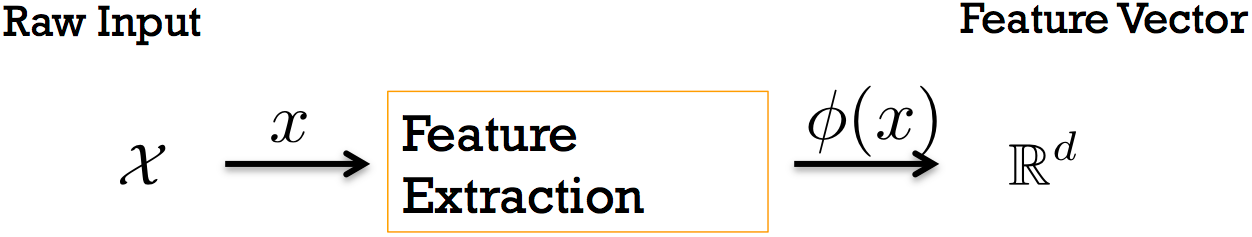
\includegraphics[width=0.9\textwidth]{figures/feature-extraction}
\par\end{center}

\end{frame}
%
\begin{frame}{Linear Models with Explicit Feature Map}
\begin{itemize}
\item Input space: $\cx$ (no assumptions)
\item Introduce \textbf{feature map} $\phi:\cx\to\reals^{d}$
\item The feature map maps into the \textbf{feature space} $\reals^{d}$.

\item Hypothesis space of affine functions on feature space:
\[
    \cf=\left\{ x\mapsto w^{T}{\color{blue}\phi(x)}+b\mid w\in\reals^{d},b\in\reals\right\} .
\]
\end{itemize}
\end{frame}
%
\begin{frame}{Geometric Example: Two class problem, nonlinear boundary}
\begin{center}
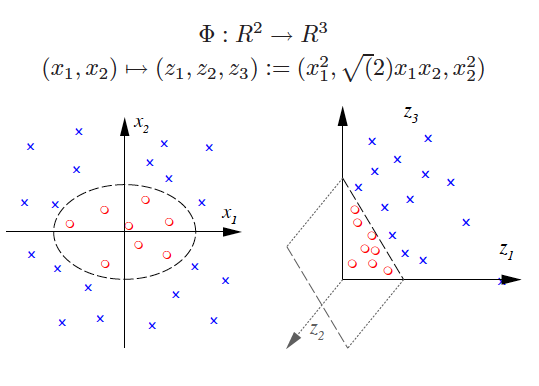
\includegraphics[height=0.6\textheight]{figures/feature-map-3d}
\par\end{center}
    \vspace{-1em}
\begin{itemize}
\item With identity feature map $\phi(x)=\left(x_{1},x_{2}\right)$ and
linear models, can't separate regions

\item With appropriate featurization $\phi(x)=\left(x_{1},x_{2},x_{1}^{2}+x_{2}^{2}\right)$,
becomes linearly separable . 

\item Video: \url{http://youtu.be/3liCbRZPrZA} 
\end{itemize}
    \let\thefootnote\relax\footnotetext{\tiny{\url{https://math.stackexchange.com/questions/353607/how-do-inner-product-space-determine-half-planes}}}
\end{frame}
%
\begin{frame}{Expressivity of Hypothesis Space}
\begin{itemize}
\item For linear models, to grow the hypothesis spaces, we must add features.

\item Sometimes we say a larger hypothesis is \hl{more expressive}. 
\begin{itemize}
\item (can fit more relationships between input and action)
\end{itemize}

\item Many ways to create new features.
\end{itemize}
\end{frame}
%

\section{Handling Nonlinearity with Linear Methods}
\begin{frame}{Example Task: Predicting Health}
\begin{itemize}
\item General Philosophy: Extract every feature that might be relevant

\item Features for medical diagnosis
\begin{itemize}
\item height
\item weight
\item body temperature
\item blood pressure
\item etc...
\end{itemize}
\end{itemize}
\let\thefootnote\relax\footnotetext{\tiny{From Percy Liang's "Lecture 3" slides from Stanford's CS221, Autumn 2014. }}
\end{frame}

\begin{frame}{Feature Issues for Linear Predictors}
\begin{itemize}
\item For linear predictors, it's important \textbf{how} features are added
    \begin{itemize}
        \item The relation between a feature and the label may not be linear
        \item There may be complex dependence among features
    \end{itemize}

\item Three types of nonlinearities can cause problems:

\begin{itemize}
\item Non-monotonicity
\item Saturation
\item Interactions between features
\end{itemize}
\end{itemize}
\let\thefootnote\relax\footnotetext{\tiny{From Percy Liang's "Lecture 3" slides from Stanford's CS221, Autumn 2014. }}
\end{frame}

\begin{frame}{Non-monotonicity: The Issue}
\begin{itemize}
\item Feature Map: $\phi(x)=\left[1,\text{temperature}(x)\right]$

\item Action: Predict health score $y\in\reals$ (positive is good)

\item Hypothesis Space $\cf{=}\left\{ \mbox{affine functions of temperature}\right\} $

\item Issue: 

\begin{itemize}
\item Health is not an affine function of temperature.

\item Affine function can either say
\begin{itemize}
\item Very high is bad and very low is good, or
\item Very low is bad and very high is good,
\item But here, both extremes are bad.
\end{itemize}
\end{itemize}
\end{itemize}
\let\thefootnote\relax\footnotetext{\tiny{From Percy Liang's "Lecture 3" slides from Stanford's CS221, Autumn 2014. }}
\end{frame}

\begin{frame}{Non-monotonicity: Solution 1}
\begin{itemize}
\item Transform the input:
\[
\phi(x)=\left[1,\left\{ \text{temperature(x)-37}\right\} ^{2}\right],
\]
where $37$ is ``normal'' temperature in Celsius.

\item Ok, but requires manually-specified domain knowledge
\begin{itemize}
\item Do we really need that?
\item What does $w^T\phi(x)$ look like?
\end{itemize}
\end{itemize}
\let\thefootnote\relax\footnotetext{\tiny{From Percy Liang's "Lecture 3" slides from Stanford's CS221, Autumn 2014. }}
\end{frame}

\begin{frame}{Non-monotonicity: Solution 2}
\begin{itemize}
\item Think less, put in more:
\[
\phi(x)=\left[1,\text{temperature}(x),\left\{ \text{temperature}(x)\right\} ^{2}\right].
\]


\item \hl{More expressive} than Solution 1.

\end{itemize}
\begin{block}{General Rule}

Features should be simple building blocks that can be pieced together.
\end{block}
\let\thefootnote\relax\footnotetext{\tiny{From Percy Liang's "Lecture 3" slides from Stanford's CS221, Autumn 2014. }}
\end{frame}

\begin{frame}{Saturation: The Issue}
\begin{itemize}
\item Setting: Find products relevant to user's query

\item Input: Product $x$
\item Action: Score the relevance of $x$ to user's query

\item Feature Map:
\[
\phi(x)=\left[1,N(x)\right],
\]
where $N(x)=\text{number of people who bought }x$.

\item We expect a monotonic relationship between $N(x)$ and relevance,
    but also expect \hl{diminishing return}.
\end{itemize}
\let\thefootnote\relax\footnotetext{\tiny{From Percy Liang's "Lecture 3" slides from Stanford's CS221, Autumn 2014. }}
\end{frame}

\begin{frame}{Saturation: Solve with nonlinear transform}
\begin{itemize}
\item Smooth nonlinear transformation:
\[
\phi(x)=\left[1,\log\left\{ 1+N(x)\right\} \right]
\]

        \begin{itemize}
    \item $\log\left(\cdot\right)$ good for values with large dynamic ranges
    \end{itemize}
\item Discretization (a discontinuous transformation):
\[
\phi(x)=\left(\ind{0\le N(x)<10},\ind{10\le N(x)<100},\ldots\right)
\]

        \begin{itemize}
\item Small buckets allow quite flexible relationship
        \end{itemize}

\end{itemize}
\let\thefootnote\relax\footnotetext{\tiny{From Percy Liang's "Lecture 3" slides from Stanford's CS221, Autumn 2014. }}
\end{frame}

\begin{frame}{Interactions: The Issue}
\begin{itemize}
\item Input: Patient information $x$
\item Action: Health score $y\in\reals$ (higher is better)
\item Feature Map
\[
\phi(x)=\left[\mbox{height}(x),\mbox{weight}(x)\right]
\]


\item Issue: It's the weight \textit{relative} to the height that's important.

\item Impossible to get with these features and a linear classifier.
\item Need some \textbf{interaction} between height and weight.

\let\thefootnote\relax\footnotetext{\tiny{From Percy Liang's "Lecture 3" slides from Stanford's CS221, Autumn 2014. }}
\end{itemize}
\end{frame}

\begin{frame}{Interactions: Approach 1}
\begin{itemize}
\item Google ``ideal weight from height''

\item J. D. Robinson's ``ideal weight'' formula (for a male):
\[
\mbox{weight}\mbox{(kg)}=52+1.9\left[\mbox{height(in)}-60\right]
\]


\item Make score square deviation between height($h$) and ideal weight($w$)
\[
f(x)=\left(52+1.9\left[h(x)-60\right]-w(x)\right)^{2}
\]


\item WolframAlpha for complicated Mathematics:
\[
f(x)=3.61h(x)^{2}-3.8h(x)w(x)-235.6h(x)+w(x)^{2}+124w(x)+3844
\]
\end{itemize}
\let\thefootnote\relax\footnotetext{\tiny{From Percy Liang's "Lecture 3" slides from Stanford's CS221, Autumn 2014. }}
\end{frame}

\begin{frame}{Interactions: Approach 2}
\begin{itemize}
\item Just include all second order features:
\[
\phi(x)=\left[1,h(x),w(x),h(x)^{2},w(x)^{2},\underbrace{h(x)w(x)}_{\mbox{cross term}}\right]
\]

\item More flexible, no Google, no WolframAlpha.
\end{itemize}
\begin{block}{General Principle}

Simpler building blocks replace a single ``smart'' feature.
\end{block}
\let\thefootnote\relax\footnotetext{\tiny{From Percy Liang's "Lecture 3" slides from Stanford's CS221, Autumn 2014. }}
\end{frame}

%\begin{frame}{Predicate Features and Interaction Terms}
%\begin{definition}
%A \textbf{predicate} on the input space $\cx$ is a function $P:\cx\to\left\{ \mbox{True},\mbox{False}\right\} $.
%
%\pause{}
%\end{definition}
%
%\begin{itemize}
%\item Many features take this form:
%\begin{itemize}
%\item $x\mapsto s(x)=\ind{\mbox{subject is sleeping}}$
%\item $x\mapsto d(x)=\ind{\mbox{subject is driving}}$
%
%\pause{}
%\end{itemize}
%\item For predicates, interaction terms correspond to \textbf{AND} conjunctions:
%\begin{itemize}
%\item $x\mapsto s(x)d(x)=\ind{\mbox{subject is sleeping AND subject is driving}}$
%\end{itemize}
%\end{itemize}
%\let\thefootnote\relax\footnotetext{\tiny{From Percy Liang's "Lecture 3" slides from Stanford's CS221, Autumn 2014. }}
%\end{frame}

\begin{frame}{Monomial Interaction Terms}
    \textbf{Interaction terms} are useful building blocks to model non-linearities in features.
\begin{itemize}
\item Suppose we start with $x=\left(1,x_{1},\ldots,x_{d}\right)\in\reals^{d+1}=\cx$.

\item Consider adding all \textbf{monomials} of degree $M$: $x_{1}^{p_{1}}\cdots x_{d}^{p_{d}}$,
with $p_{1}+\cdots+p_{d}=M$.
        \begin{itemize}
            \item Monomials with degree 2 in 2D space: $x_1^2$, $x_2^2$, $x_1x_2$
        \end{itemize}
\item How many features will we end up with? ${M+d-1 \choose M}$ (``stars and bars'')
\item This leads to extremely \al{large data matrices}
\begin{itemize}
\item For $d=40$ and $M=8$, we get $314457495$ features.
\end{itemize}
\end{itemize}
\end{frame}
%
\begin{frame}{Big Feature Spaces}

Very large feature spaces have two potential issues:\\
\begin{itemize}
\item Overfitting
\item Memory and computational costs 
\end{itemize}

    Solutions:\\
\begin{itemize}
\item Overfitting we handle with regularization.
\item \textbf{Kernel methods} can help with memory and
    computational costs when we go to high (or infinite) dimensional spaces.
\end{itemize}
\end{frame}


\end{document}
